\documentclass[]{article}
\usepackage{lmodern}
\usepackage{amssymb,amsmath}
\usepackage{ifxetex,ifluatex}
\usepackage{fixltx2e} % provides \textsubscript
\ifnum 0\ifxetex 1\fi\ifluatex 1\fi=0 % if pdftex
  \usepackage[T1]{fontenc}
  \usepackage[utf8]{inputenc}
\else % if luatex or xelatex
  \ifxetex
    \usepackage{mathspec}
  \else
    \usepackage{fontspec}
  \fi
  \defaultfontfeatures{Ligatures=TeX,Scale=MatchLowercase}
\fi
% use upquote if available, for straight quotes in verbatim environments
\IfFileExists{upquote.sty}{\usepackage{upquote}}{}
% use microtype if available
\IfFileExists{microtype.sty}{%
\usepackage{microtype}
\UseMicrotypeSet[protrusion]{basicmath} % disable protrusion for tt fonts
}{}
\usepackage[margin=1in]{geometry}
\usepackage{hyperref}
\hypersetup{unicode=true,
            pdftitle={R Programming Hw4},
            pdfauthor={Amy Fox},
            pdfborder={0 0 0},
            breaklinks=true}
\urlstyle{same}  % don't use monospace font for urls
\usepackage{color}
\usepackage{fancyvrb}
\newcommand{\VerbBar}{|}
\newcommand{\VERB}{\Verb[commandchars=\\\{\}]}
\DefineVerbatimEnvironment{Highlighting}{Verbatim}{commandchars=\\\{\}}
% Add ',fontsize=\small' for more characters per line
\usepackage{framed}
\definecolor{shadecolor}{RGB}{248,248,248}
\newenvironment{Shaded}{\begin{snugshade}}{\end{snugshade}}
\newcommand{\AlertTok}[1]{\textcolor[rgb]{0.94,0.16,0.16}{#1}}
\newcommand{\AnnotationTok}[1]{\textcolor[rgb]{0.56,0.35,0.01}{\textbf{\textit{#1}}}}
\newcommand{\AttributeTok}[1]{\textcolor[rgb]{0.77,0.63,0.00}{#1}}
\newcommand{\BaseNTok}[1]{\textcolor[rgb]{0.00,0.00,0.81}{#1}}
\newcommand{\BuiltInTok}[1]{#1}
\newcommand{\CharTok}[1]{\textcolor[rgb]{0.31,0.60,0.02}{#1}}
\newcommand{\CommentTok}[1]{\textcolor[rgb]{0.56,0.35,0.01}{\textit{#1}}}
\newcommand{\CommentVarTok}[1]{\textcolor[rgb]{0.56,0.35,0.01}{\textbf{\textit{#1}}}}
\newcommand{\ConstantTok}[1]{\textcolor[rgb]{0.00,0.00,0.00}{#1}}
\newcommand{\ControlFlowTok}[1]{\textcolor[rgb]{0.13,0.29,0.53}{\textbf{#1}}}
\newcommand{\DataTypeTok}[1]{\textcolor[rgb]{0.13,0.29,0.53}{#1}}
\newcommand{\DecValTok}[1]{\textcolor[rgb]{0.00,0.00,0.81}{#1}}
\newcommand{\DocumentationTok}[1]{\textcolor[rgb]{0.56,0.35,0.01}{\textbf{\textit{#1}}}}
\newcommand{\ErrorTok}[1]{\textcolor[rgb]{0.64,0.00,0.00}{\textbf{#1}}}
\newcommand{\ExtensionTok}[1]{#1}
\newcommand{\FloatTok}[1]{\textcolor[rgb]{0.00,0.00,0.81}{#1}}
\newcommand{\FunctionTok}[1]{\textcolor[rgb]{0.00,0.00,0.00}{#1}}
\newcommand{\ImportTok}[1]{#1}
\newcommand{\InformationTok}[1]{\textcolor[rgb]{0.56,0.35,0.01}{\textbf{\textit{#1}}}}
\newcommand{\KeywordTok}[1]{\textcolor[rgb]{0.13,0.29,0.53}{\textbf{#1}}}
\newcommand{\NormalTok}[1]{#1}
\newcommand{\OperatorTok}[1]{\textcolor[rgb]{0.81,0.36,0.00}{\textbf{#1}}}
\newcommand{\OtherTok}[1]{\textcolor[rgb]{0.56,0.35,0.01}{#1}}
\newcommand{\PreprocessorTok}[1]{\textcolor[rgb]{0.56,0.35,0.01}{\textit{#1}}}
\newcommand{\RegionMarkerTok}[1]{#1}
\newcommand{\SpecialCharTok}[1]{\textcolor[rgb]{0.00,0.00,0.00}{#1}}
\newcommand{\SpecialStringTok}[1]{\textcolor[rgb]{0.31,0.60,0.02}{#1}}
\newcommand{\StringTok}[1]{\textcolor[rgb]{0.31,0.60,0.02}{#1}}
\newcommand{\VariableTok}[1]{\textcolor[rgb]{0.00,0.00,0.00}{#1}}
\newcommand{\VerbatimStringTok}[1]{\textcolor[rgb]{0.31,0.60,0.02}{#1}}
\newcommand{\WarningTok}[1]{\textcolor[rgb]{0.56,0.35,0.01}{\textbf{\textit{#1}}}}
\usepackage{graphicx,grffile}
\makeatletter
\def\maxwidth{\ifdim\Gin@nat@width>\linewidth\linewidth\else\Gin@nat@width\fi}
\def\maxheight{\ifdim\Gin@nat@height>\textheight\textheight\else\Gin@nat@height\fi}
\makeatother
% Scale images if necessary, so that they will not overflow the page
% margins by default, and it is still possible to overwrite the defaults
% using explicit options in \includegraphics[width, height, ...]{}
\setkeys{Gin}{width=\maxwidth,height=\maxheight,keepaspectratio}
\IfFileExists{parskip.sty}{%
\usepackage{parskip}
}{% else
\setlength{\parindent}{0pt}
\setlength{\parskip}{6pt plus 2pt minus 1pt}
}
\setlength{\emergencystretch}{3em}  % prevent overfull lines
\providecommand{\tightlist}{%
  \setlength{\itemsep}{0pt}\setlength{\parskip}{0pt}}
\setcounter{secnumdepth}{0}
% Redefines (sub)paragraphs to behave more like sections
\ifx\paragraph\undefined\else
\let\oldparagraph\paragraph
\renewcommand{\paragraph}[1]{\oldparagraph{#1}\mbox{}}
\fi
\ifx\subparagraph\undefined\else
\let\oldsubparagraph\subparagraph
\renewcommand{\subparagraph}[1]{\oldsubparagraph{#1}\mbox{}}
\fi

%%% Use protect on footnotes to avoid problems with footnotes in titles
\let\rmarkdownfootnote\footnote%
\def\footnote{\protect\rmarkdownfootnote}

%%% Change title format to be more compact
\usepackage{titling}

% Create subtitle command for use in maketitle
\newcommand{\subtitle}[1]{
  \posttitle{
    \begin{center}\large#1\end{center}
    }
}

\setlength{\droptitle}{-2em}

  \title{R Programming Hw4}
    \pretitle{\vspace{\droptitle}\centering\huge}
  \posttitle{\par}
    \author{Amy Fox}
    \preauthor{\centering\large\emph}
  \postauthor{\par}
      \predate{\centering\large\emph}
  \postdate{\par}
    \date{October 24, 2018}


\begin{document}
\maketitle

\begin{Shaded}
\begin{Highlighting}[]
\NormalTok{knitr}\OperatorTok{::}\NormalTok{opts_chunk}\OperatorTok{$}\KeywordTok{set}\NormalTok{(}\DataTypeTok{message =} \OtherTok{FALSE}\NormalTok{)}
\end{Highlighting}
\end{Shaded}

Load necessary packages

\begin{Shaded}
\begin{Highlighting}[]
\KeywordTok{library}\NormalTok{(readr)}
\KeywordTok{library}\NormalTok{(tidyr)}
\KeywordTok{library}\NormalTok{(dplyr)}
\KeywordTok{library}\NormalTok{(forcats)}
\KeywordTok{library}\NormalTok{(broom)}
\KeywordTok{library}\NormalTok{(purrr)}
\KeywordTok{library}\NormalTok{(ggplot2)}
\KeywordTok{library}\NormalTok{(knitr)}
\end{Highlighting}
\end{Shaded}

Read in homicide csv

\begin{Shaded}
\begin{Highlighting}[]
\NormalTok{homicides <-}\StringTok{ }\KeywordTok{read_csv}\NormalTok{(}\StringTok{"../data/homicide-data.csv"}\NormalTok{)}
\end{Highlighting}
\end{Shaded}

See first few lines of data to see what's there

\begin{Shaded}
\begin{Highlighting}[]
\KeywordTok{head}\NormalTok{(homicides)}
\end{Highlighting}
\end{Shaded}

\begin{verbatim}
## # A tibble: 6 x 12
##   uid        reported_date victim_last victim_first victim_race victim_age
##   <chr>              <int> <chr>       <chr>        <chr>       <chr>     
## 1 Alb-000001      20100504 GARCIA      JUAN         Hispanic    78        
## 2 Alb-000002      20100216 MONTOYA     CAMERON      Hispanic    17        
## 3 Alb-000003      20100601 SATTERFIELD VIVIANA      White       15        
## 4 Alb-000004      20100101 MENDIOLA    CARLOS       Hispanic    32        
## 5 Alb-000005      20100102 MULA        VIVIAN       White       72        
## 6 Alb-000006      20100126 BOOK        GERALDINE    White       91        
## # ... with 6 more variables: victim_sex <chr>, city <chr>, state <chr>,
## #   lat <dbl>, lon <dbl>, disposition <chr>
\end{verbatim}

Unite the city and state columns to make a general location column\\
Remove Tulsa, AL because does not exist and skews data

\begin{Shaded}
\begin{Highlighting}[]
\NormalTok{homicides <-}\StringTok{ }\NormalTok{homicides }\OperatorTok
\StringTok{  }\KeywordTok{unite}\NormalTok{(}\DataTypeTok{col =} \StringTok{"location"}\NormalTok{, }\KeywordTok{c}\NormalTok{(}\StringTok{"city"}\NormalTok{, }\StringTok{"state"}\NormalTok{),}
        \DataTypeTok{sep =} \StringTok{", "}\NormalTok{) }\OperatorTok
\StringTok{  }\KeywordTok{filter}\NormalTok{(location }\OperatorTok{!=}\StringTok{"Tulsa, AL"}\NormalTok{)}
\end{Highlighting}
\end{Shaded}

\emph{Key for myself}\\
\emph{unsolved = closed without arrest or open/no arrest}

Create new dataframe with unsolved cases info\\
Select only necessary columns\\
Make a new True/False column for unsolved cases\\
Group by the location and summarize the number of unsolved and the total
cases

\begin{Shaded}
\begin{Highlighting}[]
\NormalTok{unsolved_df <-}\StringTok{ }\NormalTok{homicides }\OperatorTok
\StringTok{  }\KeywordTok{select}\NormalTok{(location, disposition) }\OperatorTok
\StringTok{  }\KeywordTok{mutate}\NormalTok{(}\DataTypeTok{unsolved =}\NormalTok{ disposition }\OperatorTok{!=}\StringTok{ "Closed by arrest"}\NormalTok{) }\OperatorTok
\StringTok{  }\KeywordTok{group_by}\NormalTok{(location) }\OperatorTok
\StringTok{  }\KeywordTok{summarise}\NormalTok{(}\DataTypeTok{total_cases =} \KeywordTok{n}\NormalTok{(), }\DataTypeTok{unsolved =} \KeywordTok{sum}\NormalTok{(unsolved))}

\KeywordTok{head}\NormalTok{(unsolved_df)}
\end{Highlighting}
\end{Shaded}

\begin{verbatim}
## # A tibble: 6 x 3
##   location        total_cases unsolved
##   <chr>                 <int>    <int>
## 1 Albuquerque, NM         378      146
## 2 Atlanta, GA             973      373
## 3 Baltimore, MD          2827     1825
## 4 Baton Rouge, LA         424      196
## 5 Birmingham, AL          800      347
## 6 Boston, MA              614      310
\end{verbatim}

Create new dataframe with only data for Baltimore\\
Perform proportion test on Baltimore cases\\
Tidy prop\_test data

\begin{Shaded}
\begin{Highlighting}[]
\NormalTok{Baltimore_df <-}\StringTok{ }\NormalTok{unsolved_df }\OperatorTok
\StringTok{  }\KeywordTok{filter}\NormalTok{(location }\OperatorTok{==}\StringTok{ "Baltimore, MD"}\NormalTok{)}

\NormalTok{Baltimore_prop_test <-}\StringTok{ }\KeywordTok{prop.test}\NormalTok{(}\DataTypeTok{x=}\NormalTok{ Baltimore_df}\OperatorTok{$}\NormalTok{unsolved, }
                                  \DataTypeTok{n =}\NormalTok{ Baltimore_df}\OperatorTok{$}\NormalTok{total_cases)}

\CommentTok{#print output of prop.test}
\NormalTok{Baltimore_prop_test}
\end{Highlighting}
\end{Shaded}

\begin{verbatim}
## 
##  1-sample proportions test with continuity correction
## 
## data:  Baltimore_df$unsolved out of Baltimore_df$total_cases, null probability 0.5
## X-squared = 239.01, df = 1, p-value < 2.2e-16
## alternative hypothesis: true p is not equal to 0.5
## 95 percent confidence interval:
##  0.6275625 0.6631599
## sample estimates:
##         p 
## 0.6455607
\end{verbatim}

\begin{Shaded}
\begin{Highlighting}[]
\CommentTok{# print tidied prop.test}
\NormalTok{tidied_Baltimore_prop_test <-}\StringTok{ }\KeywordTok{tidy}\NormalTok{(Baltimore_prop_test)}
\NormalTok{tidied_Baltimore_prop_test}
\end{Highlighting}
\end{Shaded}

\begin{verbatim}
##    estimate statistic      p.value parameter  conf.low conf.high
## 1 0.6455607   239.011 6.461911e-54         1 0.6275625 0.6631599
##                                                 method alternative
## 1 1-sample proportions test with continuity correction   two.sided
\end{verbatim}

\begin{Shaded}
\begin{Highlighting}[]
\CommentTok{#pull out estimate proportion and confidence intervals}
\NormalTok{tidied_Baltimore_prop_test}\OperatorTok{$}\NormalTok{estimate}
\end{Highlighting}
\end{Shaded}

\begin{verbatim}
## [1] 0.6455607
\end{verbatim}

\begin{Shaded}
\begin{Highlighting}[]
\NormalTok{tidied_Baltimore_prop_test}\OperatorTok{$}\NormalTok{conf.low}
\end{Highlighting}
\end{Shaded}

\begin{verbatim}
## [1] 0.6275625
\end{verbatim}

\begin{Shaded}
\begin{Highlighting}[]
\NormalTok{tidied_Baltimore_prop_test}\OperatorTok{$}\NormalTok{conf.high}
\end{Highlighting}
\end{Shaded}

\begin{verbatim}
## [1] 0.6631599
\end{verbatim}

Create new column with prop.test of each city using map2\\
Create new column with tidied proptest data\\
Unnest data --\textgreater{} tidy data from list to df\\
Reorder location by estimate

Plot cities according to the estimate for unsolved cases showing the
95\% confidence interval\\
Change x axis from decimal to percent\\
Add labels

(Must change fig.width to fig\_width for PDF)

\begin{Shaded}
\begin{Highlighting}[]
\NormalTok{tidy_cities_prop <-}\StringTok{ }\NormalTok{unsolved_df }\OperatorTok
\StringTok{  }\KeywordTok{mutate}\NormalTok{(}\DataTypeTok{my_prop_test =} \KeywordTok{map2}\NormalTok{(unsolved, total_cases, prop.test),}
         \DataTypeTok{tidy_prop_test =} \KeywordTok{map}\NormalTok{(my_prop_test, tidy)) }\OperatorTok
\StringTok{  }\KeywordTok{unnest}\NormalTok{(tidy_prop_test, }\DataTypeTok{.drop =} \OtherTok{TRUE}\NormalTok{) }\OperatorTok
\StringTok{  }\KeywordTok{mutate}\NormalTok{(}\DataTypeTok{location =} \KeywordTok{factor}\NormalTok{(location, }\DataTypeTok{levels =}\NormalTok{ location[}\KeywordTok{order}\NormalTok{(estimate)]))}
  

\NormalTok{tidy_cities_prop }\OperatorTok
\KeywordTok{ggplot}\NormalTok{(}\KeywordTok{aes}\NormalTok{(estimate, location)) }\OperatorTok{+}
\StringTok{  }\KeywordTok{geom_point}\NormalTok{(}\DataTypeTok{color =} \StringTok{"white"}\NormalTok{) }\OperatorTok{+}
\StringTok{  }\KeywordTok{geom_errorbarh}\NormalTok{(}\KeywordTok{aes}\NormalTok{(}\DataTypeTok{xmin =}\NormalTok{ conf.low, }
                     \DataTypeTok{xmax =}\NormalTok{ conf.high, }
                     \DataTypeTok{height =} \DecValTok{0}\NormalTok{),  }\DataTypeTok{color =} \StringTok{"white"}\NormalTok{) }\OperatorTok{+}
\StringTok{  }\KeywordTok{scale_x_continuous}\NormalTok{(}\DataTypeTok{labels=}\NormalTok{ scales}\OperatorTok{::}\NormalTok{percent) }\OperatorTok{+}
\StringTok{  }\KeywordTok{ggtitle}\NormalTok{(}\StringTok{"Unsolved homicides by city"}\NormalTok{, }\DataTypeTok{subtitle =} \StringTok{"Bars show 95% confidence interval"}\NormalTok{) }\OperatorTok{+}
\StringTok{  }\KeywordTok{xlab}\NormalTok{(}\StringTok{"Percent of homicdes that are unsolved"}\NormalTok{)}\OperatorTok{+}
\StringTok{  }\KeywordTok{ylab}\NormalTok{(}\StringTok{""}\NormalTok{) }\OperatorTok{+}
\StringTok{  }\KeywordTok{theme_dark}\NormalTok{()}
\end{Highlighting}
\end{Shaded}

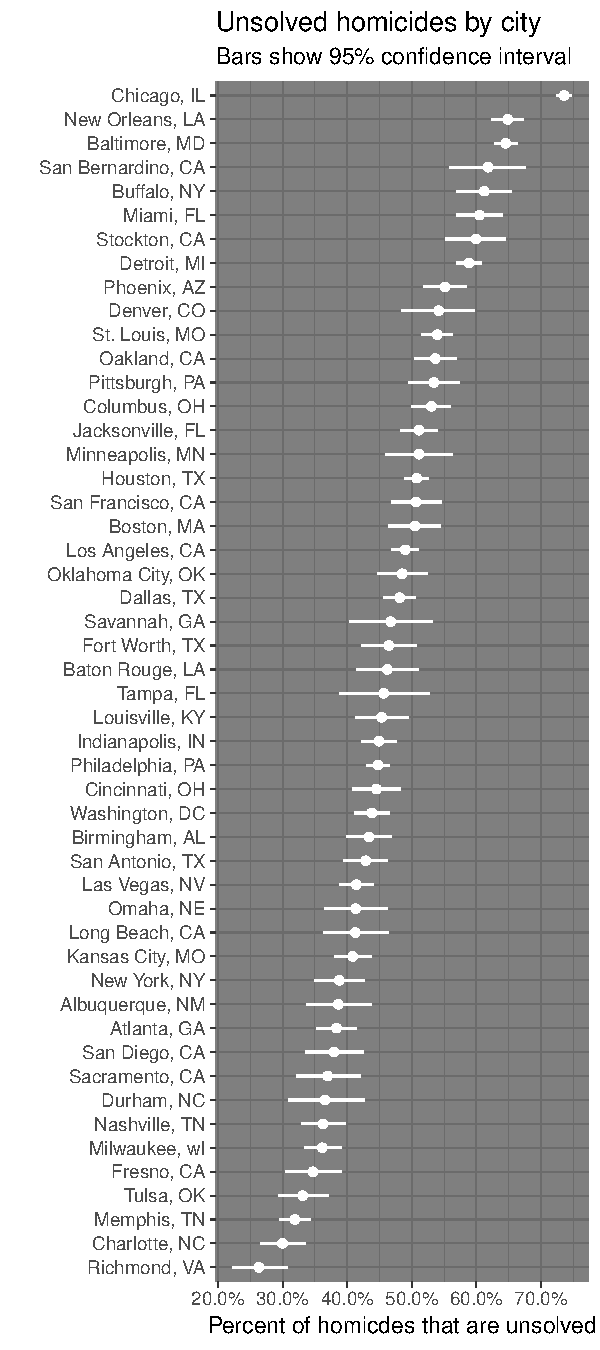
\includegraphics{Hw4_files/figure-latex/unnamed-chunk-8-1.pdf}


\end{document}
